\chapter{Risultati}
\label{cap:risultati}

\section{Esperimenti su PC}
\label{sec:esperimenti-su-pc}

In questa sezione discutiamo i risultati degli esperimenti sui modelli proposti condotti in ambiente PC; innanzitutto analizziamo le migliori metriche ottenute dalla classificazione delle attività e degli utenti sia per il dataset costruito ad hoc che per il dataset DLA, in seguito studiamo le performance al variare della lunghezza della finestra di processing e delle feature calcolate ed infine mostriamo alcuni test di significatività parametrici.

\subsection{Metriche d'accuratezza}
\label{ssec:metriche-di-accuratezza}

Nella Tabella \ref{tab:activity-classification} possiamo vedere i risultati delle metriche ottenute dai quattro classificatori proposti sia sul dataset costruito ad hoc che sul dataset DLA; questi valori fanno riferimento ai migliori risultati ricavati da ogni modello durante un esperimento di 5-fold cross-validation variando la lunghezza della finestra di campionamento e, per i modelli classici, il numero di features; per ogni metrica è riportato in grassetto il miglior risultato fra i quattro modelli.

Nel caso del dataset ad hoc il classificatore SVM produce il miglior valore per la metrica di Recall (0.934), mentre LSTM ottiene la migliore Accuracy (0.947) e ERS-KNN produce le migliori Precision e F1-score(0.941 e 0.936); questo ci mostra come la classificazione dei lavaggi e delle sanificazioni attraverso segnali raccolti da smartwatch comuni sia un processo fattibile sia con gli strumenti standard di machine learning che con quelli più avanzati di deep learning. L'attività di sanificazione è quella con i risultati più bassi, circa l'82\%, ottenuta da CNN; questo è probabilmente dato dal fatto che le sanificazioni sono attività meno dinamiche rispetto ai lavaggi, dove l'uso dell'acqua induce vibrazioni più semplici da rilevare.

Per quanto riguarda il dataset DLA il modello CNN supera gli altri modelli in ogni metrica calcolata, nonostante questo le performance di ERS-KNN rimangono sopra al 91\%. Paragonato agli esperimenti sul dataset ad hoc le performance hanno subito una decrescita media dal 1\% fino all'8\% a seconda del classificatore. Questa riduzione di performance può essere causata dal numero maggiore di etichette; infatti nel dataset DLA abbiamo 10 etichette totali (scrittura, lavaggio mani, lavaggio volto, lavaggio denti, spazzare, passare l'aspirapolvere, mangiare, spolverare, strofinare, altro) le quali tendono a disperdere maggiormente i risultati. Un'altra causa può essere la mancanza di segnali del giroscopio che impattano significativamente sulle capacità di classificazione, in particolare dei modelli di machine learning classici.

\begin{table}
    \centering
    \begin{tabular}{l | c c | c c | c c | c c }
        \hline
        & \multicolumn{2}{c}{SVM} & \multicolumn{2}{c}{ERS-KNN} & \multicolumn{2}{c}{CNN} & \multicolumn{2}{c}{LSTM} \\
        \hline 
        & ad hoc & DLA & ad hoc & DLA & ad hoc & DLA & ad hoc & DLA \\
        Accuracy & 0.942 & 0.891 & 0.946 & 0.914 & 0.909 & \textbf{0.923} & \textbf{0.947} & 0.866 \\
        Precision & 0.936 & 0.907 & \textbf{0.941} & 0.931 & 0.898 & \textbf{0.939} & 0.911 & 0.882 \\
        Recall & \textbf{0.934} & 0.867 & 0.932 & 0.914 & 0.917 & \textbf{0.925} & 0.908 & 0.874 \\
        F1-score& 0.935 & 0.886 & \textbf{0.936} & 0.922 & 0.908 & \textbf{0.932} & 0.910 & 0.878\\
        \hline
    \end{tabular}
    \caption{Migliori risultati della classificazione delle attività ottenuti sia dal dataset costruito ad hoc che dal dataset DLA.}
    \label{tab:activity-classification}
\end{table}

\`E importante notare che per entrambi i dataset i risultati migliori sono stati ottenuti con finestre di lunghezza: SVM=12s, ERS-KNN=8s, CNN=6s, LSTM=2s e, nel caso di SVM ed ERS-KNN, utilizzando tutte le feature.

\subsection{Riconoscimento degli utenti}
\label{ssec:riconoscimento-degli-utenti}

Il secondo insieme di esperimenti ha lo scopo di identificare la persona che lava o sanifica le mani al posto dell'attività di per sé, per questo motivo abbiamo rimosso dai dataset tutti i sample che non fanno parte di queste categorie e abbiamo cambiato le etichette per identificare la persona piuttosto che l'attività. Nella Tabella \ref{tab:person-classification} possiamo vedere le migliori metriche ottenute dai quattro classificatori su entrambi i dataset. 

Il riconoscimento degli utenti è un compito più semplice rispetto al riconoscimento delle attività; per il dataset costruito ad hoc la migliore accuratezza è dello 0.99 ottenuta con il classificatore SVM, questo indica che le attività di lavaggio e sanificazione non strutturate contengono una sorta di impronta digitale che permette la facile identificazione dell'utente che le svolge. Inoltre da questo esperimento vediamo come le tecniche di machine learning classiche superano di cinque punti percentuali quelle di deep learning. Come nel caso del dataset costruito ad hoc, anche le metriche ricavate dal dataset DLA mostrano una maggiore semplicità nel riconoscere gli utenti rispetto l'attività; in questo caso i classificatori classici superano quelli di deep learning, ma, anche se gli esperimenti hanno una buona accuratezza (sopra il 95\%), in generale si ha comunque una riduzione nelle performance rispetto al dataset costruito ad hoc.

\begin{table}
    \centering
    \begin{tabular}{l | c c | c c | c c | c c}
        \hline
        & \multicolumn{2}{c}{SVM} & \multicolumn{2}{c}{ERS-KNN} & \multicolumn{2}{c}{CNN} & \multicolumn{2}{c}{LSTM} \\
        \hline
        & ad hoc & DLA & ad hoc & DLA & ad hoc & DLA & ad hoc & DLA \\
        \hline
        Accuracy  & \textbf{0.991} & 0.946 & 0.988 & \textbf{0.959} & 0.958 & 0.941 & 0.966 & 0.902 \\
        Precision & \textbf{0.990} & 0.949 & 0.985 & \textbf{0.957} & 0.945 & 0.940 & 0.959 & 0.902 \\
        Recall    & \textbf{0.989} & 0.942 & 0.986 & \textbf{0.949} & 0.952 & 0.943 & 0.956 & 0.903 \\
        F1-score  & \textbf{0.990} & 0.946 & 0.985 & \textbf{0.959} & 0.948 & 0.939 & 0.957 & 0.903 \\
        \hline
    \end{tabular}
    \caption{Migliori risultati della classificazione degli utenti ottenuti sia dal dataset costruito ad hoc che dal dataset DLA.}
    \label{tab:person-classification}
\end{table}

\subsection{Utilizzo di memoria e tempistiche}
\label{ssec:utilizzo-di-memoria-e-tempistiche}

Per valutare la complessità dei modelli di machine learning proposti, durante ogni esperimento, abbiamo misurato le performance e l'utilizzo di memoria di ogni classificatore; in particolare, i modelli sono stati implementati nella piattaforma Matlab2021a\textsuperscript{\textregistered} utilizzando gli strumenti di machine learning integrati e sono stati eseguiti su un PC desktop con una CPU Intel\textsuperscript{\textregistered} Core i9 equipaggiata con 32GB di memoria RAM ed una GPU Nvidia\textsuperscript{\textregistered} Quadro\textsuperscript{\textregistered} RTXTM 4000. Sia la fase di addestramento che quella d'inferenza sono state svolte impostando la GPU come ambiente d'esecuzione in modo da sfruttare a pieno le potenzialità del parallelismo CUDA\textsuperscript{\textregistered}.

La Tabella \ref{tab:memory} mostra le performance e l'utilizzo di memoria di ogni modello, come atteso la fase di addestramento dei modelli di deep learning è la più lunga con un massimo di 470 secondi misurati per l'LSTM, mentre l'ERS-KNN risulta essere il più veloce da addestrare con 5.8 secondi. Dal punto di vista dell'inferenza l'SVM sorpassa di molto gli altri modelli con 160$\mu$s; è importante notare che nel caso dell'SVM e dell'ERS-KNN le tempistiche prevedono anche l'estrazione delle feature il cui costo non è trascurabile nel momento del passaggio all'esecuzione sul dispositivo embedded.

\begin{table}
    \centering
    \begin{tabular}{l c c c c}
        \hline
        & SVM & ERS-KNN & CNN & LSTM \\
        \hline
        Tempo d'addestramento(s) & 7.191 & \textbf{5.803} & 299.551  & 472.069 \\
        Tempo d'inferenza(ms) & \textbf{0.016} & 0.331 & 0.505  & 1.749 \\
        Memoria utilizzata(MB) & \textbf{4.168} & 41.996& 6.389 & 5.569 \\
        \hline
    \end{tabular}
    \caption{Tempo d'addestramento, tempo d'inferenza e memoria utilizzata dai modelli eseguiti in ambiente PC.}
    \label{tab:memory}
\end{table}

\subsection{Lunghezza della finestra}
\label{ssec:lunghezza-della-finestra}

La dimensione della finestra di processing influisce in molti modi sulla classificazione dei modelli; di seguito analizziamo nel dettaglio i risultati degli esperimenti su questa dipendenza. Sia SVM che ERS-KNN (Figura \ref{fig:window:svm} e Figura \ref{fig:window:knn}) mostrano un trend delle performance pressoché piano, anche se da un certo punto in poi le metriche iniziano a deteriorarsi; in particolare l'SVM vede un miglioramento delle performance fino ad una finestra di dimensione 12 secondi dopodiché Precision, Recall ed F1-score diminuiscono. In maniera del tutto simile, le performance dell'ERS-KNN aumentano fino ad una finestra di 8 secondi. Un trend opposto si può vedere nei risultati ottenuti dai classificatori deep learning (Figura \ref{fig:window:cnn} e Figura \ref{fig:window:lstm}), in questo caso le metriche mostrano un decremento monotono all'aumentare della finestra.

\begin{figure}[!htb]
    \centering
    \begin{subfigure}{.45\textwidth}
        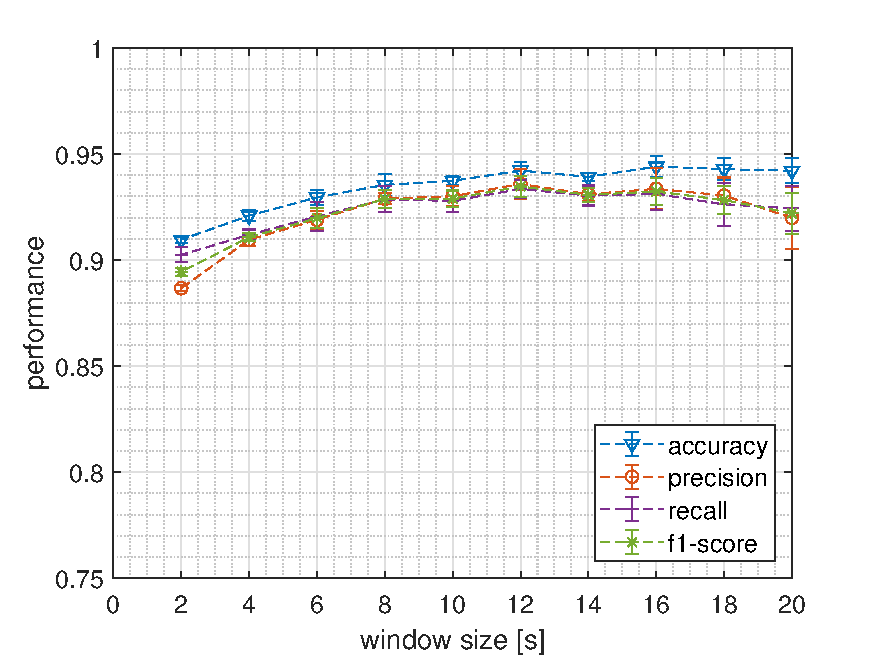
\includegraphics[width=\textwidth]{figure/svm_window.pdf}
        \caption{SVM}
        \label{fig:window:svm}
    \end{subfigure}
    \begin{subfigure}{.45\textwidth}
        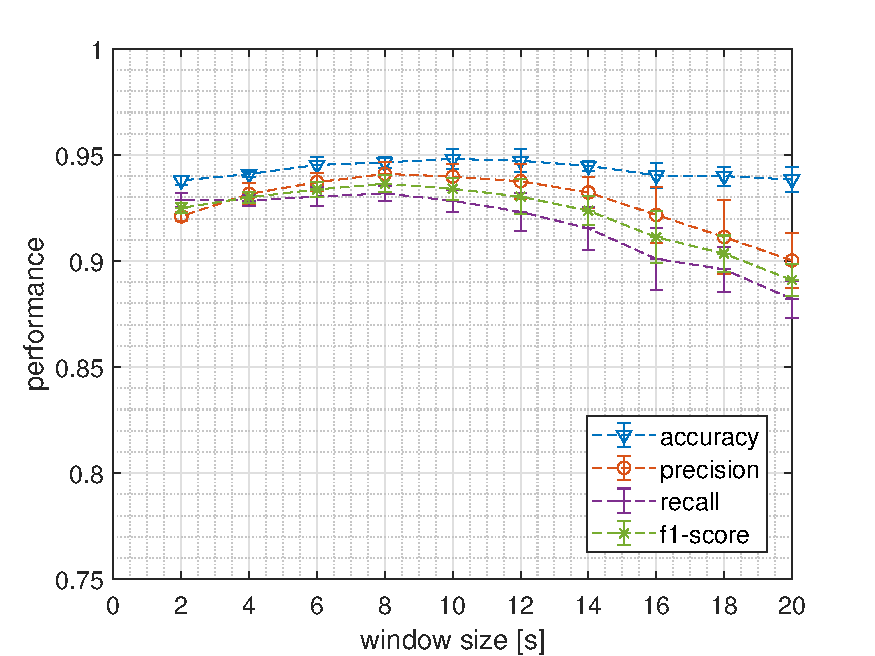
\includegraphics[width=\textwidth]{figure/knn_window.pdf}
        \caption{ERS-KNN}
        \label{fig:window:knn}
    \end{subfigure}
    \begin{subfigure}{.45\textwidth}
        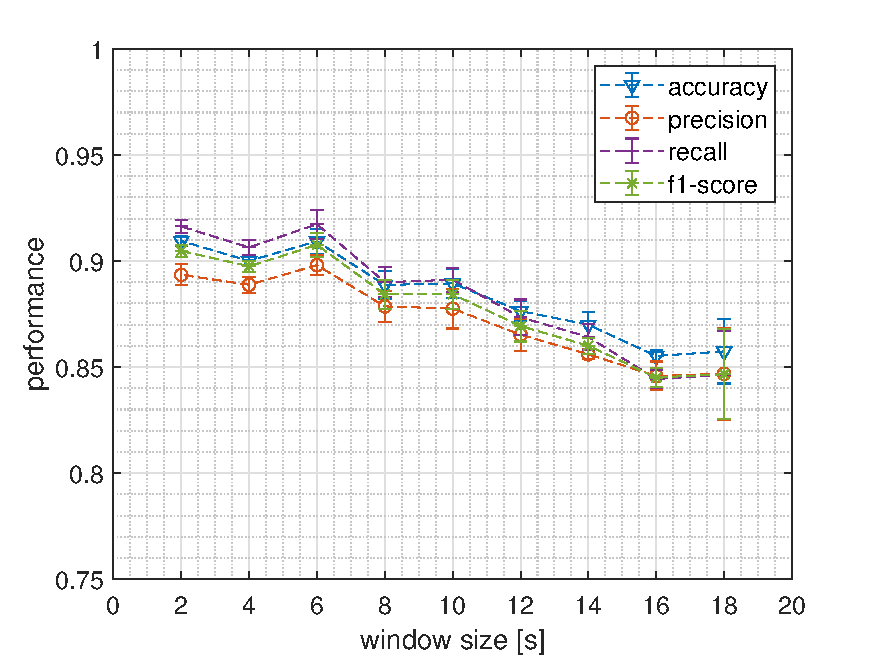
\includegraphics[width=\textwidth]{figure/cnn_window.pdf}
        \caption{CNN}
        \label{fig:window:cnn}
    \end{subfigure}
    \begin{subfigure}{.45\textwidth}
        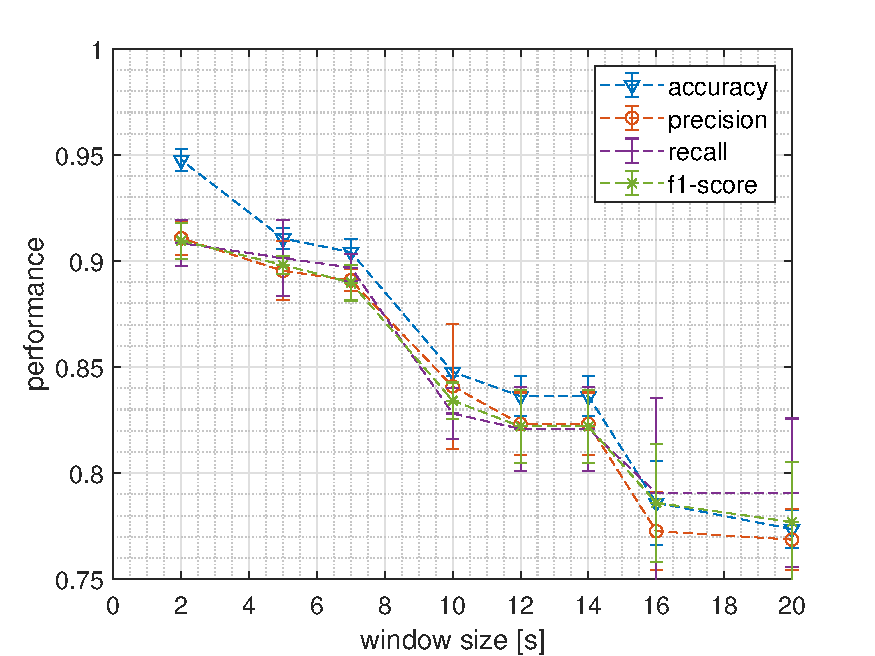
\includegraphics[width=\textwidth]{figure/lstm_window.pdf}
        \caption{LSTM}
        \label{fig:window:lstm}
    \end{subfigure}
    \caption{Performance dei modelli SVM(a), ERS-KNN(b), CNN(c) ed LSTM(d) al variare della lunghezza della finestra di processing.}
    \label{fig:window}
\end{figure}

\subsection{Selezione delle feature}
\label{ssec:selezione-delle-feature}

Oltre alla lunghezza della finestra di processing un altro parametro che influisce sulle prestazioni dei modelli di machine learning classici sono le feature che vengono calcolate. Per selezionare le feature utilizziamo un metodo detto di \textit{forward feature selection} il quale sfrutta l'accuratezza come criterio per valutare l'impatto dell'aggiunta di nuove feature partendo da un insieme vuoto fino all'esaurimento. Ogni gruppo di feature Base(B), Hjorth(H) e Shape(S) è trattato come una sola unità che può essere aggiunta o rimossa. Innanzitutto abbiamo testato i classificatori con un singolo gruppo di feature per poi aggiungere gli altri gruppi esplorando tutte le combinazioni.

La Tabella \ref{tab:features} mostra le performance per entrambi i classificatori al variare dei gruppi di feature selezionati. Le metriche mostrano tutte un aumento monotono che raggiunge le performance migliori nel momento in cui tutti i gruppi sono usati assieme; questo significa che ogni gruppo di feature aggiunge informazioni utili al processo di classificazione, inoltre, il gruppo Hjorth è quello che contiene le informazioni più utili essendo quello con  i risultati migliori dei tre gruppi quando testati da soli. 

Dal punto di vista implementativo possiamo fare un compromesso tra prestazioni e complessità computazionale scegliendo di calcolare solo le feature Base + Hjorth rinunciando allo 0.2\% delle prestazioni o, addirittura, calcolando solo le Hjorth ottenendo una precisione del 92\%, ma risparmiando molte risorse computazionali.

\begin{table}
    \centering
    \begin{tabular}{l l c c c c c c c}
        \hline
        & & B     & H     & S     & B+H   & B+S   & H+S   & B+H+S \\
        \hline
        \multirow{2}{*}{Accuracy}   & SVM & 0.901 & 0.923 & 0.339 & 0.941 & 0.916 & 0.926 & \textbf{0.942} \\
                                    & KNN & 0.904 & 0.908 & 0.719 & 0.944 & 0.908 & 0.922 & \textbf{0.946} \\
        \hline
        \multirow{2}{*}{Precision}  & SVM & 0.892 & 0.912 & 0.500 & 0.932 & 0.910 & 0.917 & \textbf{0.936} \\      
                                    & KNN & 0.899 & 0.908 & 0.683 & 0.937 & 0.909 & 0.920 & \textbf{0.941} \\
        \hline
        \multirow{2}{*}{Recall}     & SVM & 0.891 & 0.913 & 0.480 & 0.932 & 0.906 & 0.921 & \textbf{0.934} \\
                                    & KNN & 0.873 & 0.889 & 0.674 & 0.929 & 0.886 & 0.902 & \textbf{0.932} \\
        \hline
        \multirow{2}{*}{F1-score}   & SVM & 0.891 & 0.891 & 0.490 & 0.932 & 0.908 & 0.919 & \textbf{0.935} \\
                                    & KNN & 0.886 & 0.886 & 0.678 & 0.933 & 0.897 & 0.911 & \textbf{0.936} \\
        \hline
    \end{tabular}
    \caption{Risultato della selezione delle feature applicata ai due modelli di machine learning classici.}
    \label{tab:features}
\end{table}

\subsection{Test di significatività non parametrici}
\label{ssec:tesi-di-significativita-non-parametrici}

Dopo aver svolto tutti gli esperimenti sui modelli di machine learning visti in precedenza ed aver analizzato i loro risultati cerchiamo un metodo in grado di comparare questi modelli con la precisione statistica. Per questo utilizziamo tre variazioni del test di McNemar\cite{fagerland2013mcnemar}:

\begin{enumerate}
    \item test asintotico
    \item test del p-value medio
    \item test condizionale esatto
\end{enumerate}

Questo tipo di test è spesso usato in medicina per valutare gli effetti dei trattamenti, e, negli ultimi anni, nell'ambito del machine learning per comparare due modelli di grandi dimensioni senza doverli addestrare più volte. Il test di McNemar si assicura che il disaccordo fra i due casi corrisponda, commentando sul fatto che i due modelli siano in disaccordo fra loro (oppure non lo siano affatto); questo test non dice nulla sul fatto che uno dei due modelli sia più o meno accurato dell'altro.

La Tabella \ref{tab:mc-nemar-results} mostra i risultati dei tre test condotti per ogni coppia di classificatori.
Per ogni test, viene riportato il valore booleano $h$ che rappresenta la decisione del test quando si verifica l'ipotesi nulla, ovvero che i due classificatori abbiamo la stessa accuratezza nella predizione del risultato atteso.
Inoltre, viene riportato anche il valore $p$ che indica quanto è forte l'evidenza nel rifiutare o meno l'ipotesi nulla; ad esempio, quando si confrontano ERS-KNN con SVM, le tre varianti del test di McNemar concordano sull'accettare l'ipotesi nulla mentre, sia per ERS-KNN/LSTM che ERS-KNN/CNN, l'ipotesi nulla deve essere rifiutata. In questi casi, il valore $p$ per ogni test è vicino allo zero, rivelando una forte prova nel rifiutare l'ipotesi nulla.

Anche il confronto tra SVM/LSTM, SVM/CNN, e LSTM/CNN, porta a forti rifiuti dell'ipotesi nulla con p-value molto vicini allo zero, infatti, in questo scenario, solo gli strumenti di machine learning standard, ovvero SVM e ERS-KNN, possono essere considerati statisticamente equivalenti dal punto di vista delle prestazioni di classificazione.

\begin{table}
    \centering
    \begin{tabular}{c | l | c c | c c | c c }
        \hline
        & & \multicolumn{2}{c}{SVM} & \multicolumn{2}{c}{LSTM} & \multicolumn{2}{c}{CNN} \\
        \hline
                                &            & h     & p    & h    & p                      & h    & p \\
        \hline
        \multirow{3}{*}{KNN}    & asint.     & falso & $0.65$ & vero & $4.14 \times 10^{-25}$ & vero & $2.04 \times 10^{-21}$ \\
                                & p medio    & falso & $0.65$ & vero & $1.33 \times 10^{-25}$ & vero & $3.12 \times 10^{-27}$ \\
                                & esatto     & falso & $0.69$ & vero & $1.82 \times 10^{-32}$ & vero & $1.12 \times 10^{-22}$ \\
        \hline
        \multirow{3}{*}{SVM}    & asint.     &       &        & vero & $3.94 \times 10^{-05}$ & vero & $4.53 \times 10^{-22}$ \\
                                & p medio    &       &        & vero & $3.87 \times 10^{-05}$ & vero & $1.27 \times 10^{-18}$ \\
                                & esatto     &       &        & vero & $4.46 \times 10^{-05}$ & vero & $3.43 \times 10^{-22}$ \\
        \hline
        \multirow{3}{*}{LSTM}   & asint.     &       &        &      &                        & vero & $1.23 \times 10^{-25}$ \\
                                & p medio    &       &        &      &                        & vero & $5.13 \times 10^{-25}$ \\
                                & esatto     &       &        &      &                        & vero & $2.26 \times 10^{-24}$ \\ 
        \hline
    \end{tabular}
    \caption{Risultati dei tre test di McNemar sui modelli proposti.}
    \label{tab:mc-nemar-results}
\end{table}

\section{Esperimenti sull'HEXIWEAR}
\label{sec:esperimenti-sull-hexiwear}

In questa sezione discutiamo i risultati degli esperimenti condotti sui modelli proposti all'interno del dispositivo indossabile HEXIWEAR; a differenza degli esperimenti condotti su PC in questo caso viene utilizzato solo il dataset costruito ad hoc. Inizialmente analizziamo l'esito delle metriche di classificazione delle attività per il modello SVM al variare della lunghezza della finestra di processing e del numero di feature calcolate, in seguito studiamo le performance del modello LSTM al variare dei parametri interni utilizzati ed infine osserviamo le migliori prestazioni ottenute dai modelli in termini di tempo d'esecuzione, di memoria utilizzata e di consumo di energia da parte del dispositivo.

\subsection{Lunghezza della finestra di SVM}
\label{ssec:lunghezza-della-finestra-hexi}

Di seguito esaminiamo la variazione delle performance del modello SVM al variare della lunghezza della finestra di processing; la Figura \ref{fig:metrics-svm-window-hexi} mostra un cambiamento generale delle performance molto ampio con dei picchi massimi per le finestre di lunghezza 12 secondi e 14 secondi e dei picchi minimi per finestre di lunghezza 8 secondi, 10 secondi e 20 secondi, in base alle metriche. In particolare, notiamo che tutti i risultati si comportano pressoché allo stesso modo al variare della lunghezza della finestra, anche se l'accuratezza supera gli altri di sei punti percentuali, questo è sinonimo di una buona correlazione fra i valori.

\begin{figure}[!htb]
    \centering
    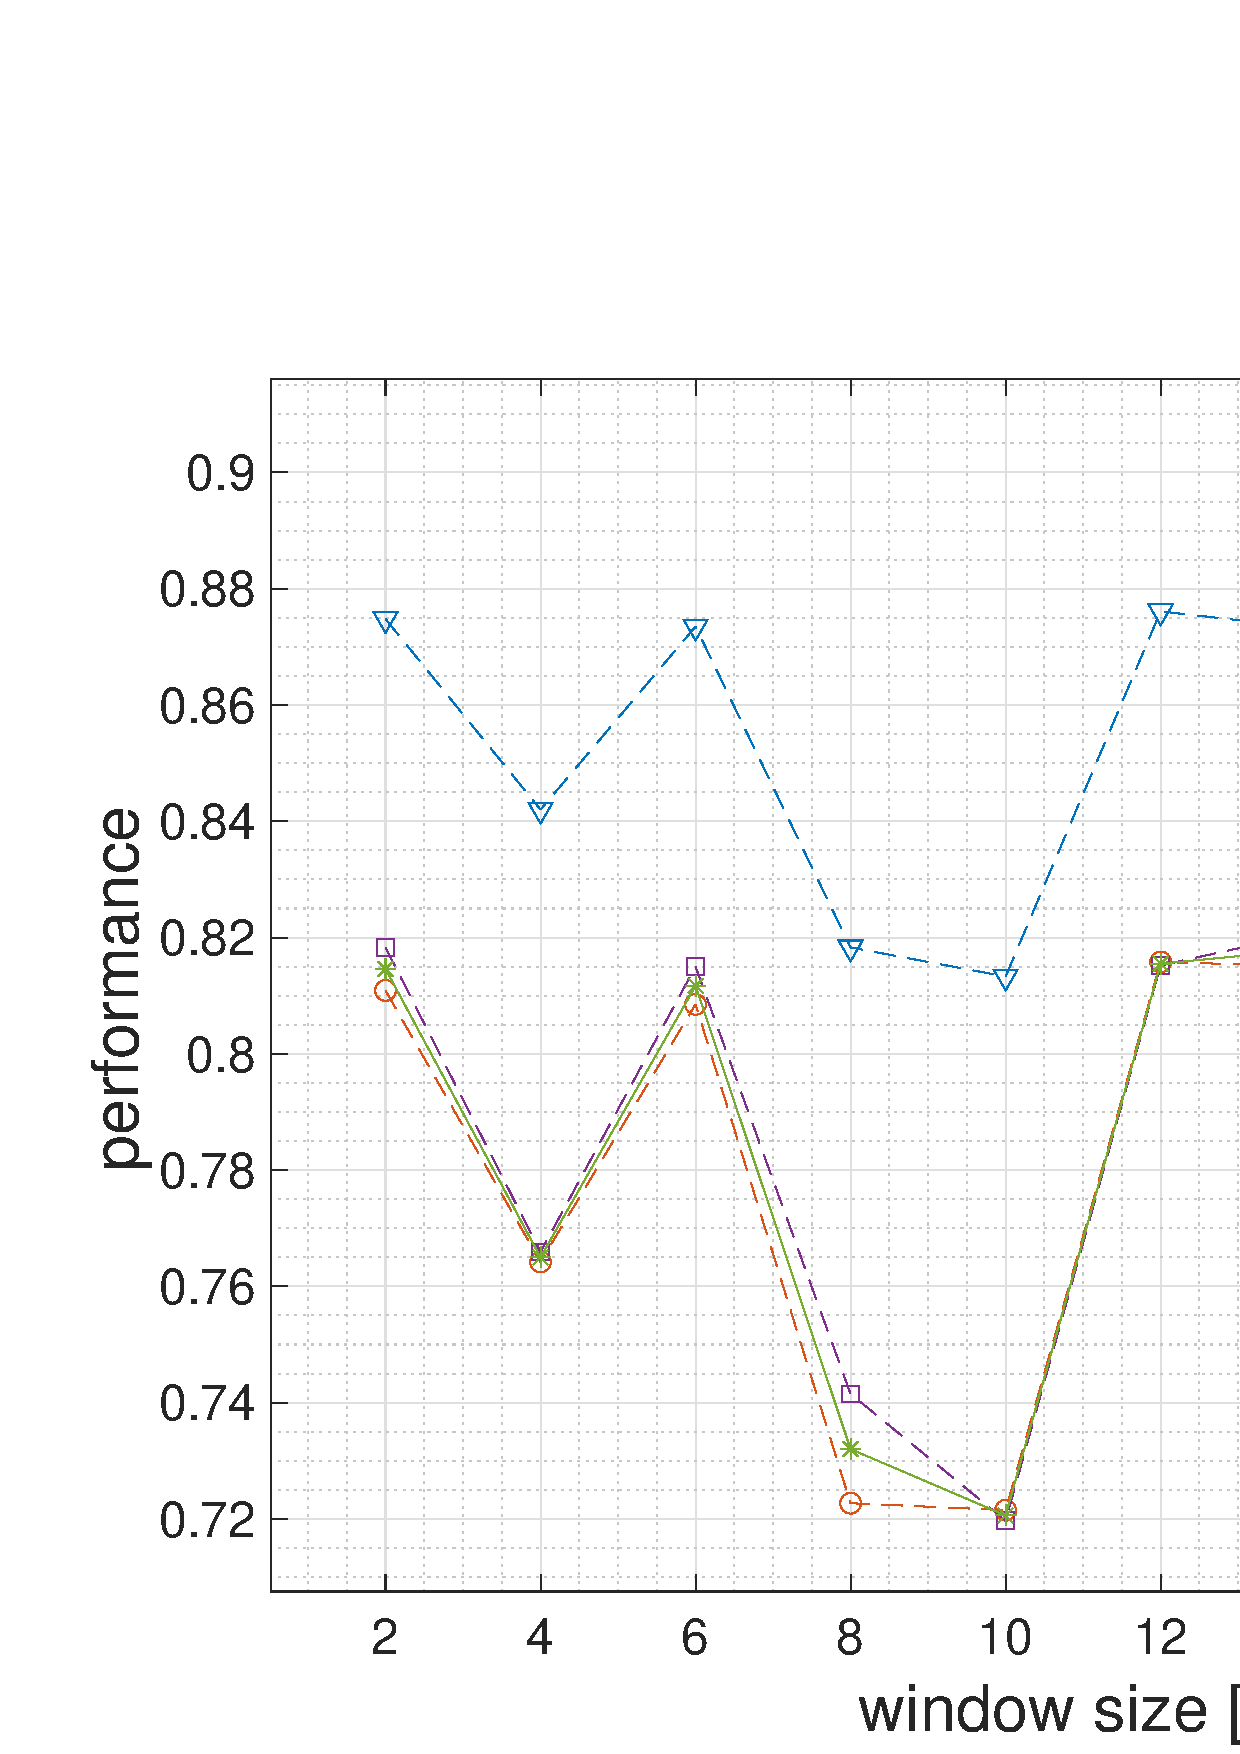
\includegraphics[width=.8\textwidth]{figure/svm_performance.pdf}
    \caption{Metriche ricavate dal modello SVM al variare della lunghezza della finestra.}
    \label{fig:metrics-svm-window-hexi}
\end{figure}

Paragonate alle performance calcolate su PC (Figura \ref{fig:window:svm}) nel caso del porting notiamo un generale peggioramento; inoltre osserviamo come su PC tutte le metriche mantengono un valore superiore al 90\% arrivando, nel caso dell'accuratezza, quasi al 95\%, mentre nel caso del porting le metriche non superano mai il 90\%, con il valore massimo dell'accuratezza al 88\%. Questo fenomeno non ci sorprende poiché è sicuramente causato dalla riduzione di capacità che abbiamo dovuto apportare ai modelli durante la fase di porting.

\subsection{Selezione delle feature di SVM}
\label{ssec:selezione-delle-feature-di-svm-hexi}

Il secondo esperimento condotto sul classificatore SVM consiste nel variare le feature calcolate ed osservare il cambiamento delle performance che ne segue. 
Come nel caso degli esperimenti condotti su PC (Sezione \ref{ssec:selezione-delle-feature}) utilizziamo il metodo di \textit{forward feature selection} per scegliere i gruppi di feature da valutare; nel porting sul dispositivo HEXIWEAR si è scelto di ridurre il numero di feature calcolate in modo da diminuire la memoria richiesta, di conseguenza le feature calcolate appartengono tutte al gruppo Base e sono: Media(A), Deviazione Standard(S), Massimo e Minimo(M).
Ogni esperimento è stato condotto utilizzando una finestra di processing di 12 secondi; per prima cosa abbiamo testato il classificatore con un singolo gruppo di feature per poi aggiungere progressivamente gli altri gruppi ed esplorare tutte le combinazioni.

La Tabella \ref{tab:metrics-svm-feat-hexi} mostra le performance al variare dei gruppi di feature calcolati; anche in questo caso le metriche presentano un aumento monotono raggiungendo le performance migliori quando tutti i gruppi sono usati assieme, poiché ogni feature aggiunge informazioni utili alla classificazione. A differenza delle altre metriche, la Recall ha un valore maggiore nel caso di \textit{Media + Deviazione Standard}; infatti questi due gruppi sono quelli che producono i risultati migliori se si esclude la combinazione di tutti tre. Inoltre il gruppo che contiene le informazioni più utili è quello della Media, producendo i risultati migliori quando preso singolarmente; mentre Deviazione Standard e Massimo e Minimo lo seguono di poco.

\begin{table}
    \centering
    \begin{tabular}{l c c c c c c c}
        \hline
        & A & S & M & A+S & A+M & S+M & A+S+M \\
        \hline
        Accuracy & 0.7946 & 0.7734 & 0.7770 & 0.8697 & 0.8589 & 0.7946 & \textbf{0.8761} \\
        Precision & 0.6638 & 0.6481 & 0.6402 & 0.7919 & 0.7818 & 0.6638 & \textbf{0.8158} \\
        Recall & 0.6682 & 0.6516 & 0.6701 & \textbf{0.8218} & 0.8021 & 0.6682 & 0.8152 \\
        F1-Score & 0.6660 & 0.6499 & 0.6548 & 0.8065 & 0.7918 & 0.6660 & \textbf{0.8155} \\
        \hline
    \end{tabular}
    \caption{Metriche ricavate dal modello SVM al variare delle feature calcolate.}
    \label{tab:metrics-svm-feat-hexi}
\end{table}

\subsection{Selezione dei parametri di LSTM}
\label{ssec:selezione-dei-parametri-di-lstm-hexi}

L'ultimo esperimento che prendiamo in esame sull'HEXIWEAR riguarda le performance del modello di deep learning LSTM variando alcuni dei suoi parametri interni. 
La rete LSTM caricata sull'HEXIWEAR (Figura \ref{fig:lstm-models-port}) è composta dal un singolo modulo LSTM e da due livelli densamente connessi; nel seguente esperimento abbiamo preso come parametri interni il numero di unità nel modulo LSTM ed il numero di neuroni nascosti all'interno del primo livello densamente connesso, mentre l'ultimo livello denso è stato settato costante pari al numero di etichette. 

In Tabella \ref{tab:metrics-lstm-param-hexi} vediamo le metriche calcolate al variare dei seguenti parametri: 64/256, 32/128, 16/64, 8/32, in cui il primo numero rappresenta il parametro del modulo LSTM ed il secondo rappresenta il numero di neuroni nello strato denso. 

Come possiamo immaginare il modello che produce i risultati migliori è quello con i parametri 64/256 con un'Accuracy dell'87\%, ed una Recall dell'88\% anche se gli altri modelli mostrano una riduzione lineare delle performance solo di circa il 3\% ad ogni riduzione dei parametri della rete.

\begin{table}
    \centering
    \begin{tabular}{l c c c c}
        \hline
        & \multicolumn{4}{c}{Parametri interni} \\
        \hline
        & 64/256 & 32/128 & 16/64 & 8/32 \\
        \hline
        Accuracy & \textbf{0.877} & 0.849 & 0.812 & 0.774 \\
        Precision & \textbf{0.879} & 0.849 & 0.809 & 0.764 \\
        Recall & \textbf{0.880} & 0.854 & 0.799 & 0.759 \\
        F1-score & \textbf{0.880} & 0.852 & 0.804 & 0.761 \\
        \hline
    \end{tabular}
    \caption{Metriche ricavate dal modello LSTM al variare dei parametri interni.}
    \label{tab:metrics-lstm-param-hexi}
\end{table}

\subsection{Utilizzo di memoria e tempistiche}
\label{ssec:utilizzo-di-memoria-e-tempistiche-hexi}

Per valutare meglio le performance complessive dei modelli di machine learning eseguiti sullo smartwatch HEXIWEAR, durante ogni esperimento abbiamo misurato le tempistiche, il consumo di memoria e l'energia di ogni classificatore.

La Tabella \ref{tab:memory-hexi} mostra i modelli con i risultati migliori fra quelli visti negli esperimenti precedenti. I parametri tempo e memoria dei sensori rappresentano il tempo in millisecondi e la memoria in byte occupati durante la fase di raccolta dei dati non elaborati dai sensori di accelerometro e giroscopio; questi due valori dipendono fortemente dalla lunghezza della finestra di processing, per questo motivo sono uguali per i due modelli SVM, che utilizzano entrambi una finestra di 12 secondi, e sono minori per il modello LSTM, che invece fa uso di una finestra di 2 secondi.

Il tempo e la memoria occupata per il calcolo delle feature sono presenti solo nei modelli SVM e, come possiamo immaginare, sono minori nel caso in cui viene calcolato un numero minore di feature. Per quanto riguarda il tempo d'inferenza notiamo una piccola differenza fra i modelli SVM, mentre il modello LSTM impiega circa il doppio del tempo, invece la memoria impiegata per l'inferenza ha valori simili fra LSTM e l'esperimento SVM con la finestra ed è minore per l'SVM con meno feature. Infine vediamo che la potenza è maggiore per il modello LSTM ed è simile fra i due modelli SVM, con l'esperimento sulle feature che ha la potenza minore.

\begin{table}
    \centering
    \begin{tabular}{l c c c}
        \hline
        & SVM window & SVM feature & LSTM \\
        \hline
        t. sensori [ms] & 10798 & 10798 & \textbf{1800} \\
        t. feature [$\mu$s] & 1161 & \textbf{226} & - \\
        t. inferenza [ms] & 52 & \textbf{48} & 85 \\
        \hline
        mem. sensori [B] & 28975 & 28975 & \textbf{4975} \\
        mem. feature [B] & 29016 & \textbf{28944} & - \\
        mem. inferenza [B] & 10398 & \textbf{4390} & 13401 \\
        mem. modello [B] & 126989 & \textbf{68625} & 111040 \\
        \hline
        potenza [mW] & 8.47 & \textbf{8.42} & 13.03 \\
        \hline
    \end{tabular}
    \caption{Tempistiche d'esecuzione, memoria utilizzata e consumo d'energia dei modelli eseguiti sul dispositivo HEXIWEAR.}
    \label{tab:memory-hexi}
\end{table}

L'ultima analisi svolta consiste nel paragonare alcune delle metriche di tempo, memoria ed energia con il valore della loss per i modelli presi in esame; la funzione loss indica il costo in termini di prestazioni del modello ed è pari ad $1 - Accuracy$.

I grafici in Figura \ref{fig:performance-svm-hexi} riportano sull'\textit{asse x} il valore della loss e sull'\textit{asse y} la memoria totale ed il consumo di energia paragonando il modello SVM dell'esperimento sulla lunghezza della finestra di processing con quello sul calcolo delle feature. 
Nei grafici memoria totale vs. loss (Figura \ref{fig:performance-svm-hexi:svm-memory-loss-window} e Figura \ref{fig:performance-svm-hexi:svm-memory-loss-feature}) vediamo che i classificatori migliori risultano essere quello con una finestra di lunghezza 2 e quello con le feature calcolate A+M, poiché sono i due ad avere un basso utilizzo di memoria mantenendo anche un valore per la loss basso; allo stesso modo nei grafici consumo d'energia vs. loss (Figura \ref{fig:performance-svm-hexi:svm-power-loss-window} e Figura \ref{fig:performance-svm-hexi:svm-power-loss-feature}) i migliori risultano essere quello con finestra di lunghezza 12 e quello con le feature calcolate A+S.

Analogamente i grafici in Figura \ref{fig:performance-lstm-hexi} confrontano il valore della loss con l'energia, il tempo d'inferenza ed il peso del modello LSTM nell'esperimento sulla variazione dei parametri interni. Come vediamo tutti e tre i grafici mostrano una repentina diminuzione dei valori all'aumentare della loss, ovvero quando vengono considerati modelli con un numero minore di parametri interni. In tutti e tre i casi il classificatore con le migliori performance rispetto alla loss risulta essere quello con 32 unità LSTM e 128 neuroni nel primo strato nascosto.

\begin{figure}[!htbp]
    \centering
    \begin{subfigure}[t]{.45\textwidth}
        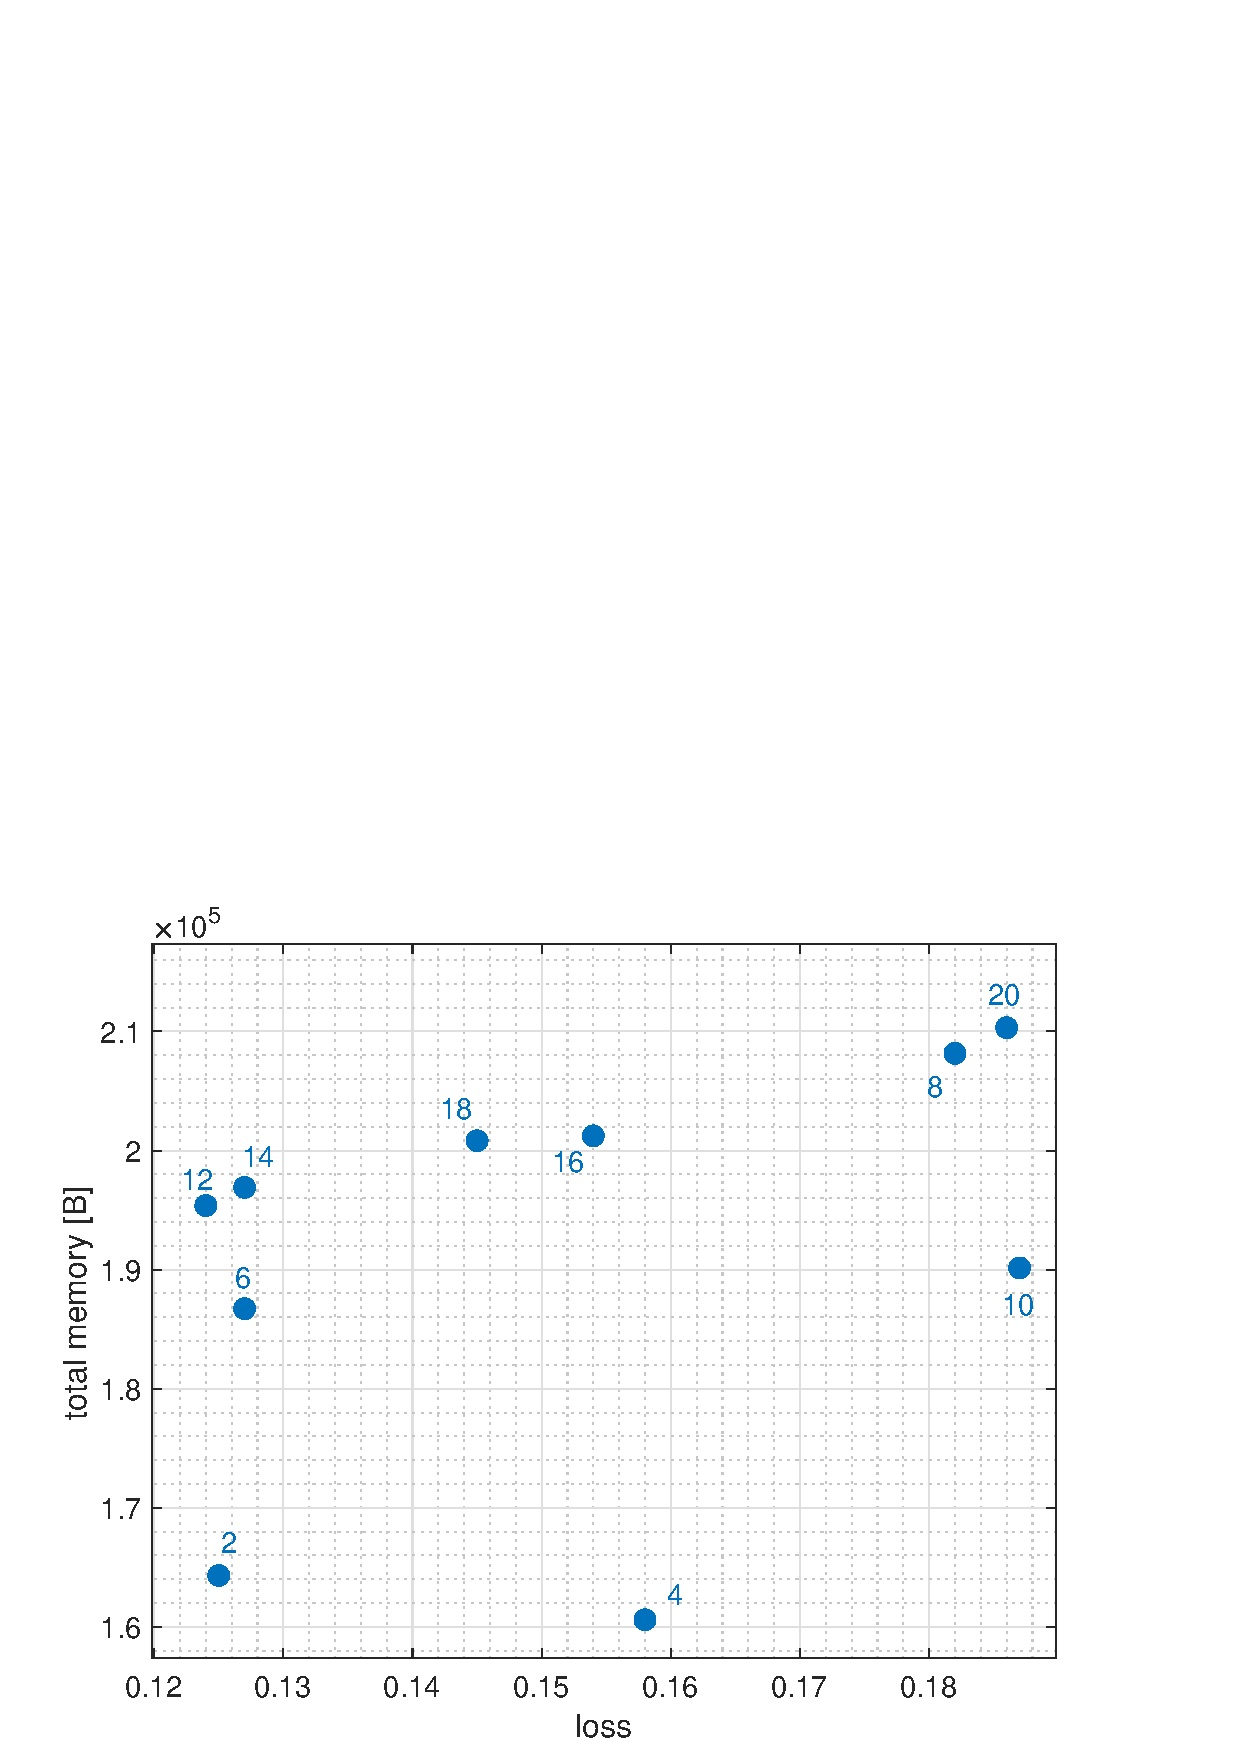
\includegraphics[width=\textwidth]{figure/svm_window_loss_memory.pdf}
        \caption{memoria totale vs. loss per gli esperimenti sulla lunghezza della finestra}
        \label{fig:performance-svm-hexi:svm-memory-loss-window}
    \end{subfigure}
    \begin{subfigure}[t]{.45\textwidth}
        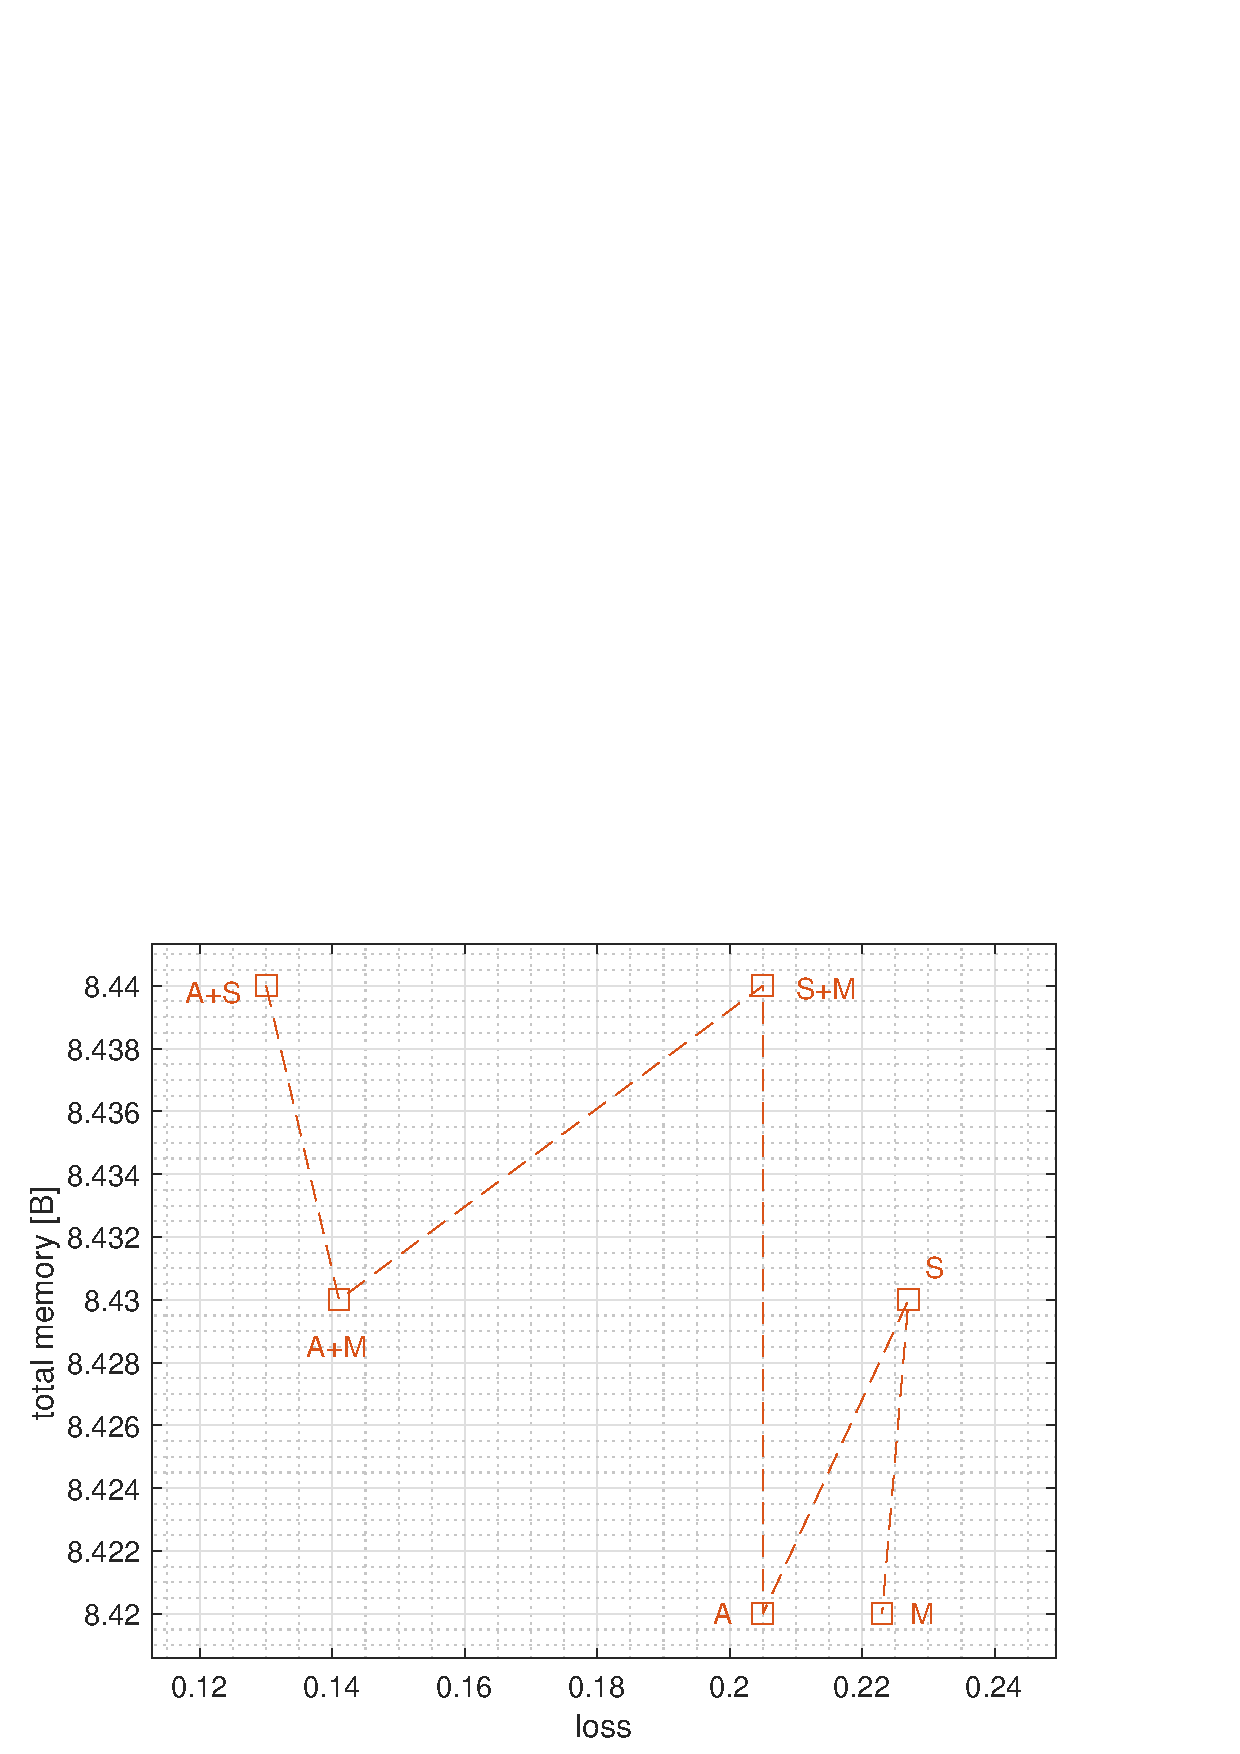
\includegraphics[width=\textwidth]{figure/svm_feat_loss_memory.pdf}
        \caption{memoria totale vs. loss per gli esperimenti sulle feature calcolate}
        \label{fig:performance-svm-hexi:svm-memory-loss-feature}
    \end{subfigure}
    \begin{subfigure}[t]{.45\textwidth}
        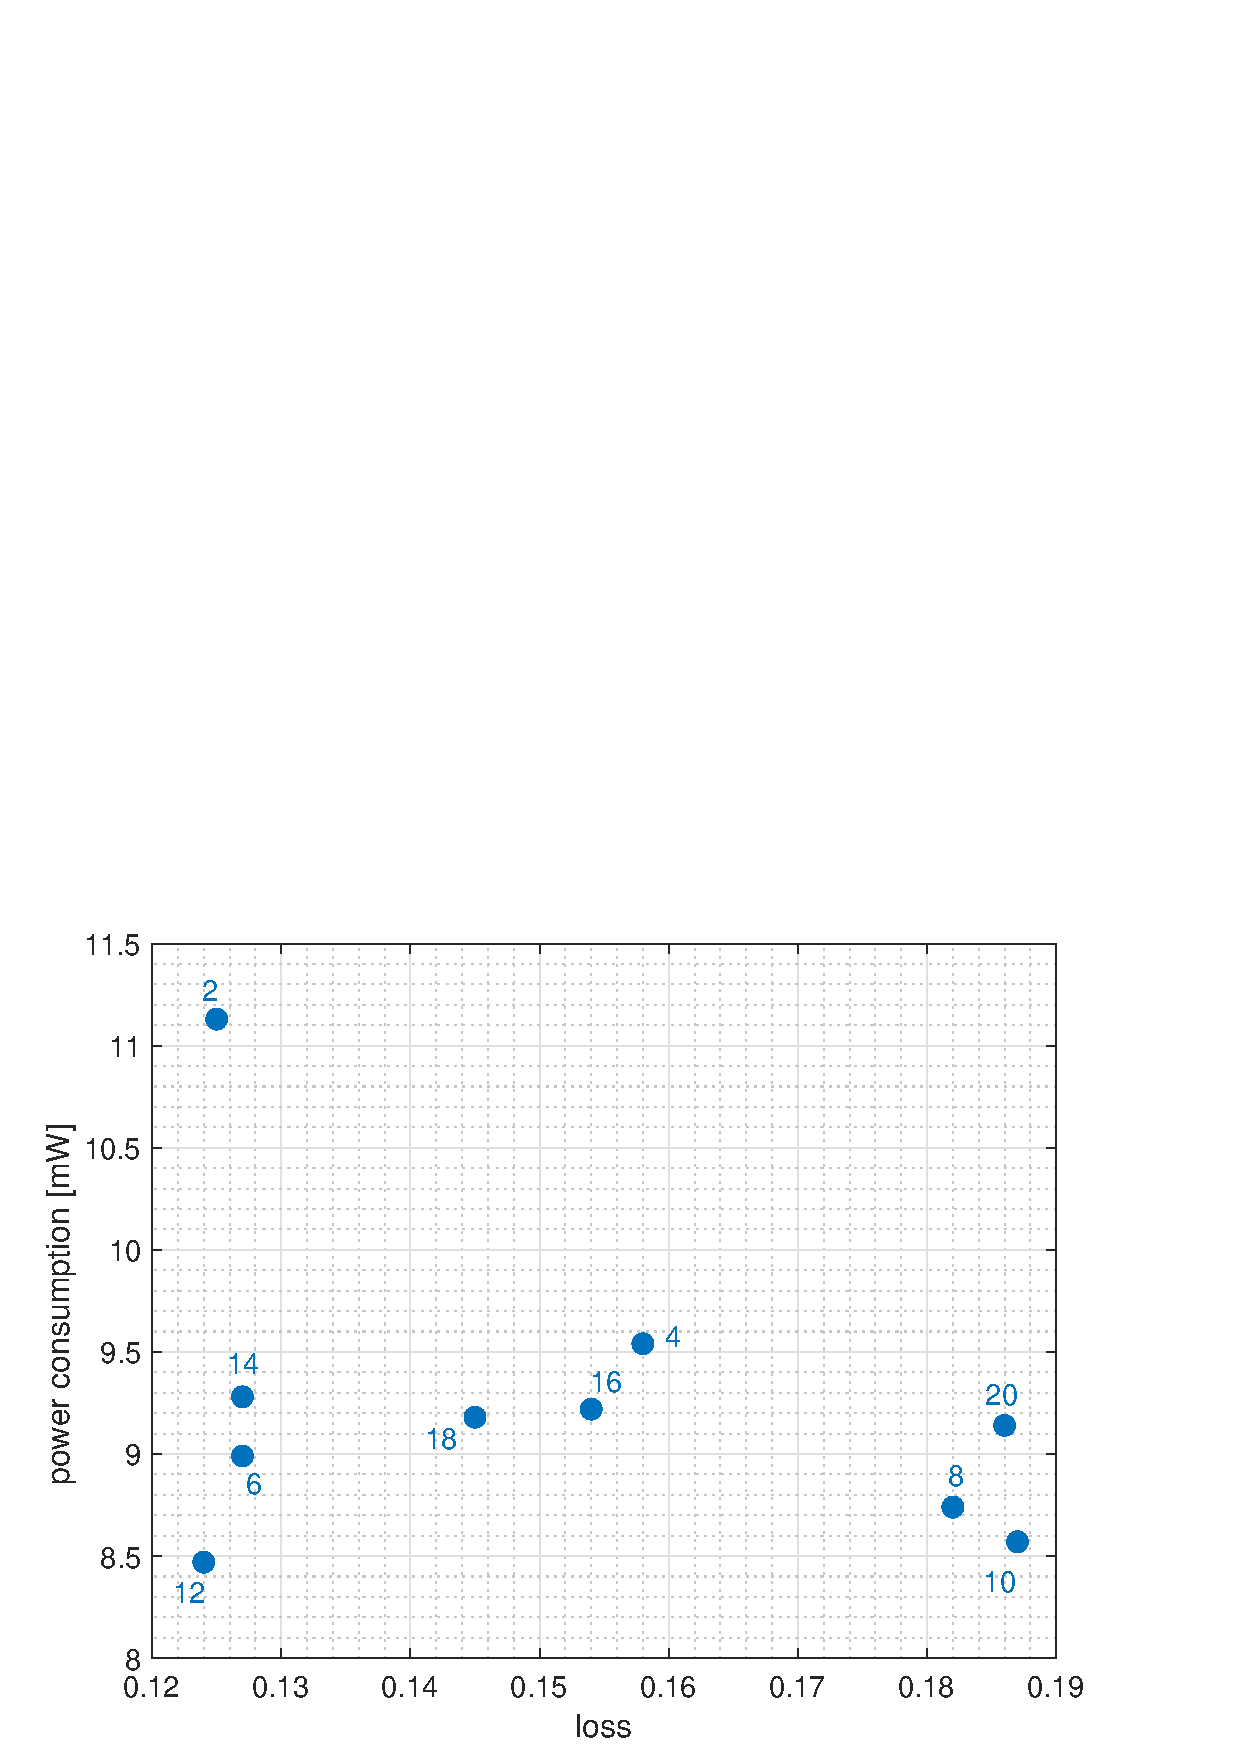
\includegraphics[width=\textwidth]{figure/svm_window_loss_power.pdf}
        \caption{consumo d'energia vs. loss per gli esperimenti sulla lunghezza della finestra}
        \label{fig:performance-svm-hexi:svm-power-loss-window}
    \end{subfigure}
    \begin{subfigure}[t]{.45\textwidth}
        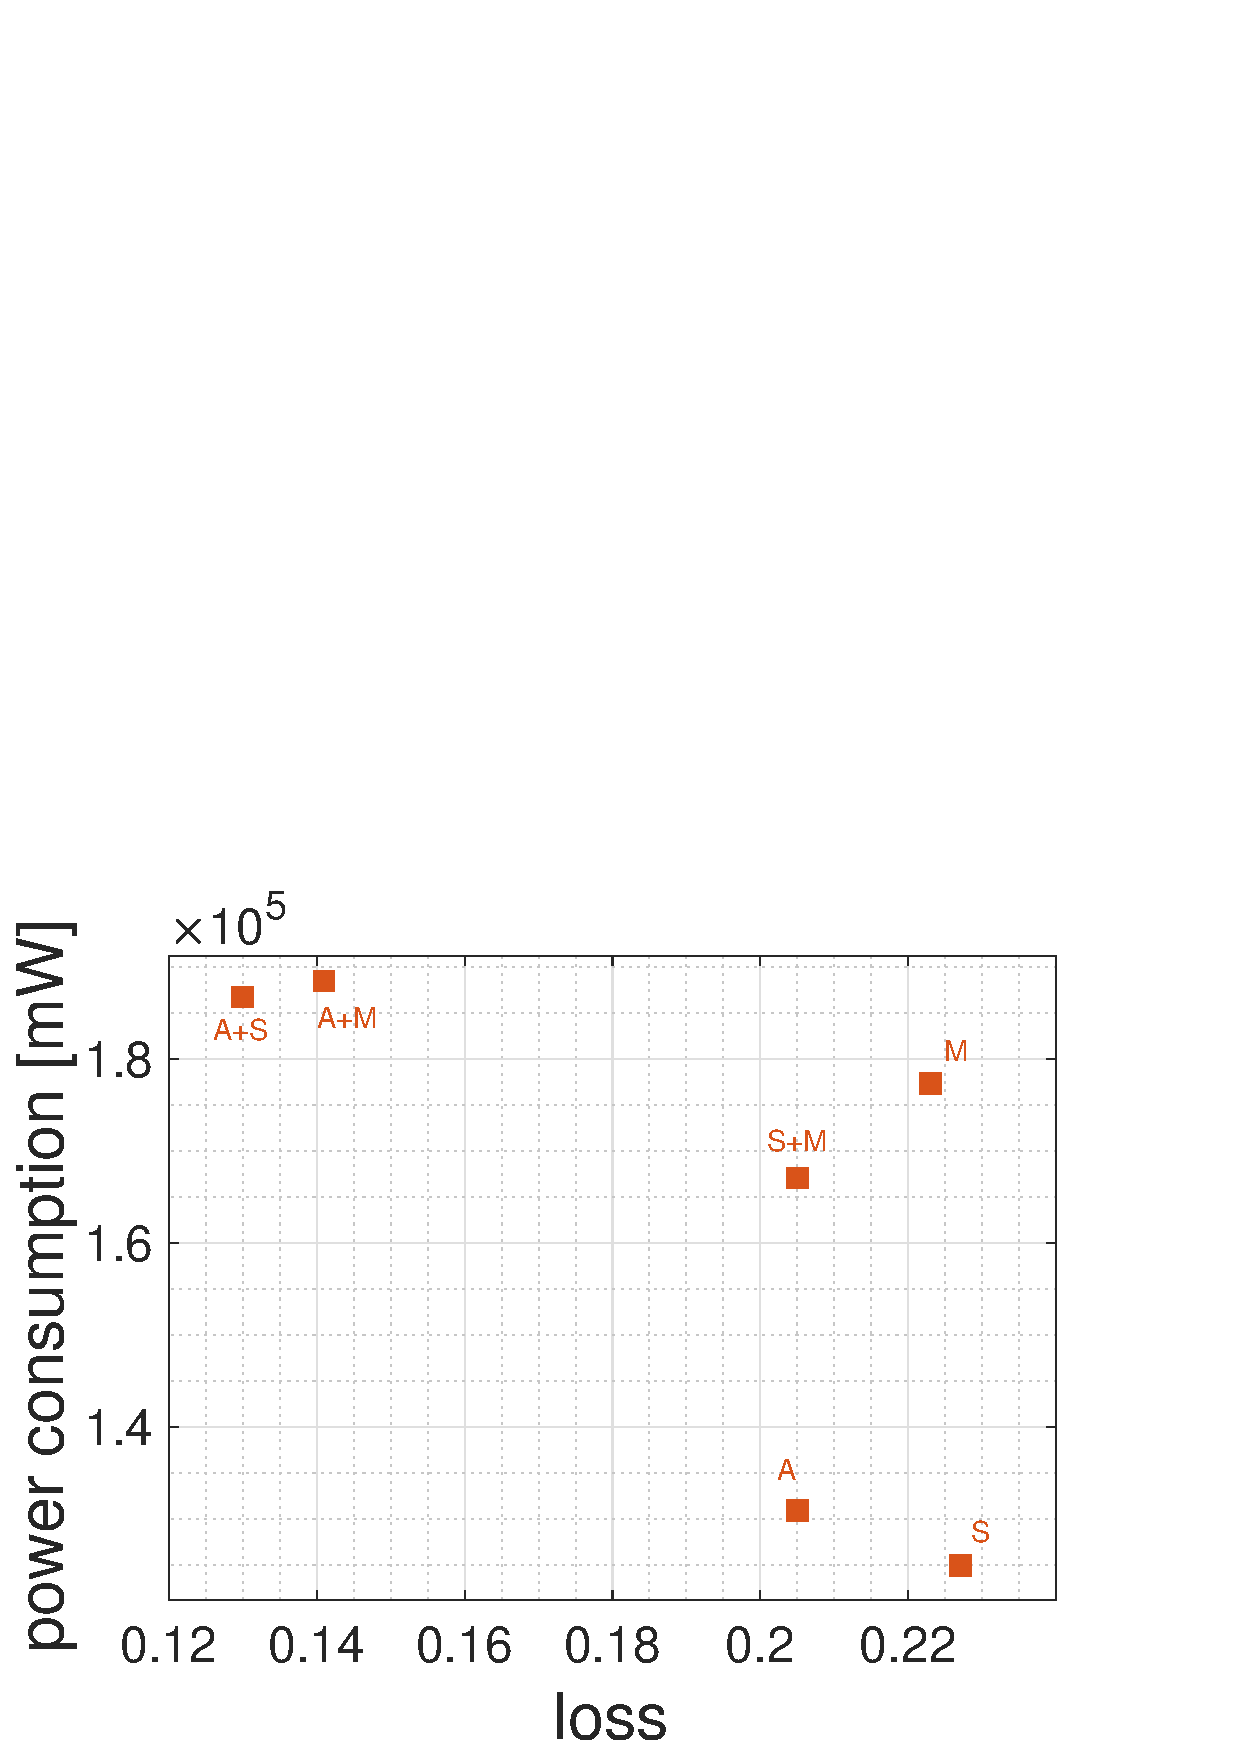
\includegraphics[width=\textwidth]{figure/svm_feat_loss_power.pdf}
        \caption{consumo d'energia vs. loss per gli esperimenti sulle feature calcolate}
        \label{fig:performance-svm-hexi:svm-power-loss-feature}
    \end{subfigure}
    \caption{Grafici prodotti dai modelli SVM confrontando memoria totale e consumo d'energia con la loss.}
    \label{fig:performance-svm-hexi}
\end{figure}

\begin{figure}[!htb]
    \centering
    \begin{subfigure}{.45\textwidth}
        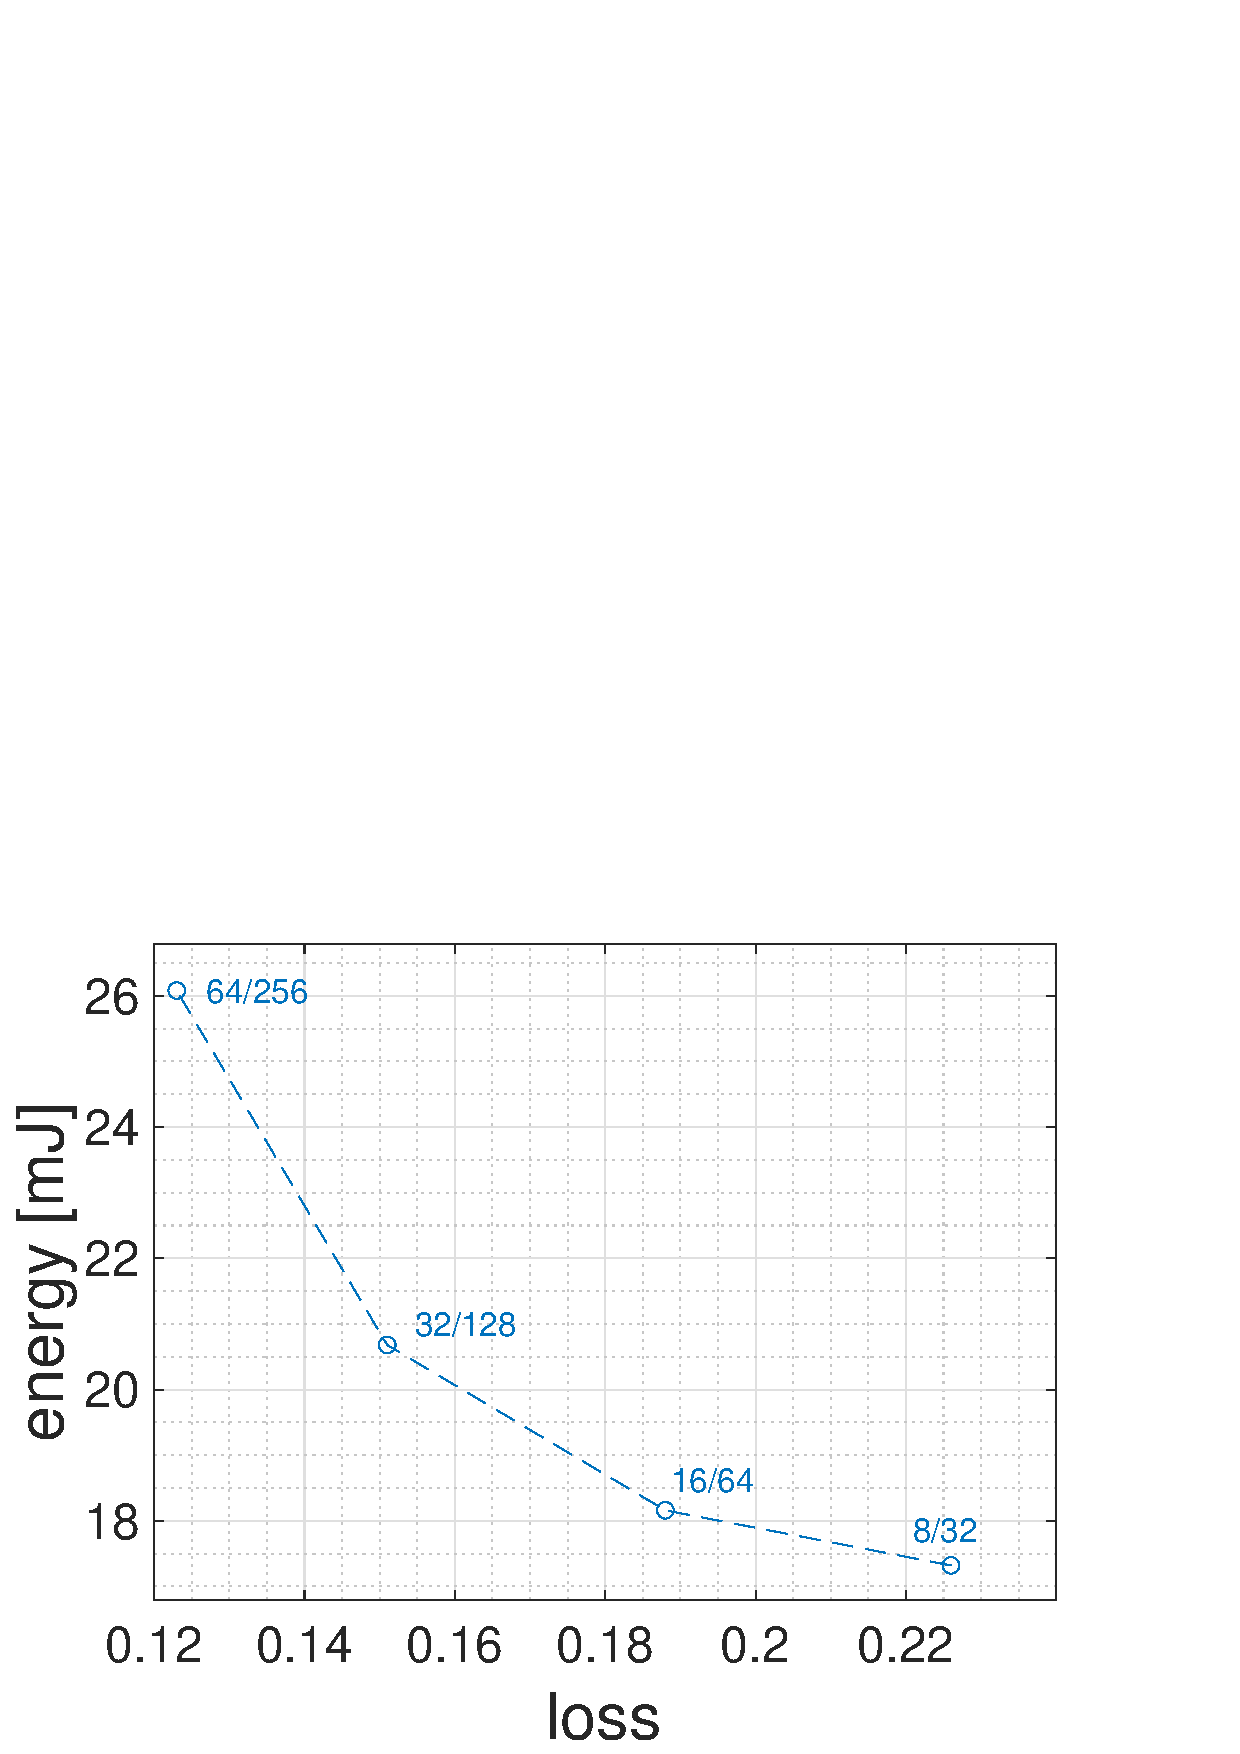
\includegraphics[width=\textwidth]{figure/lstm_energy_loss.pdf}
        \caption{consumo di energia vs. loss}
        \label{fig:performance-lstm-hexi:lstm-energy-loss}
    \end{subfigure}
    \begin{subfigure}{.45\textwidth}
        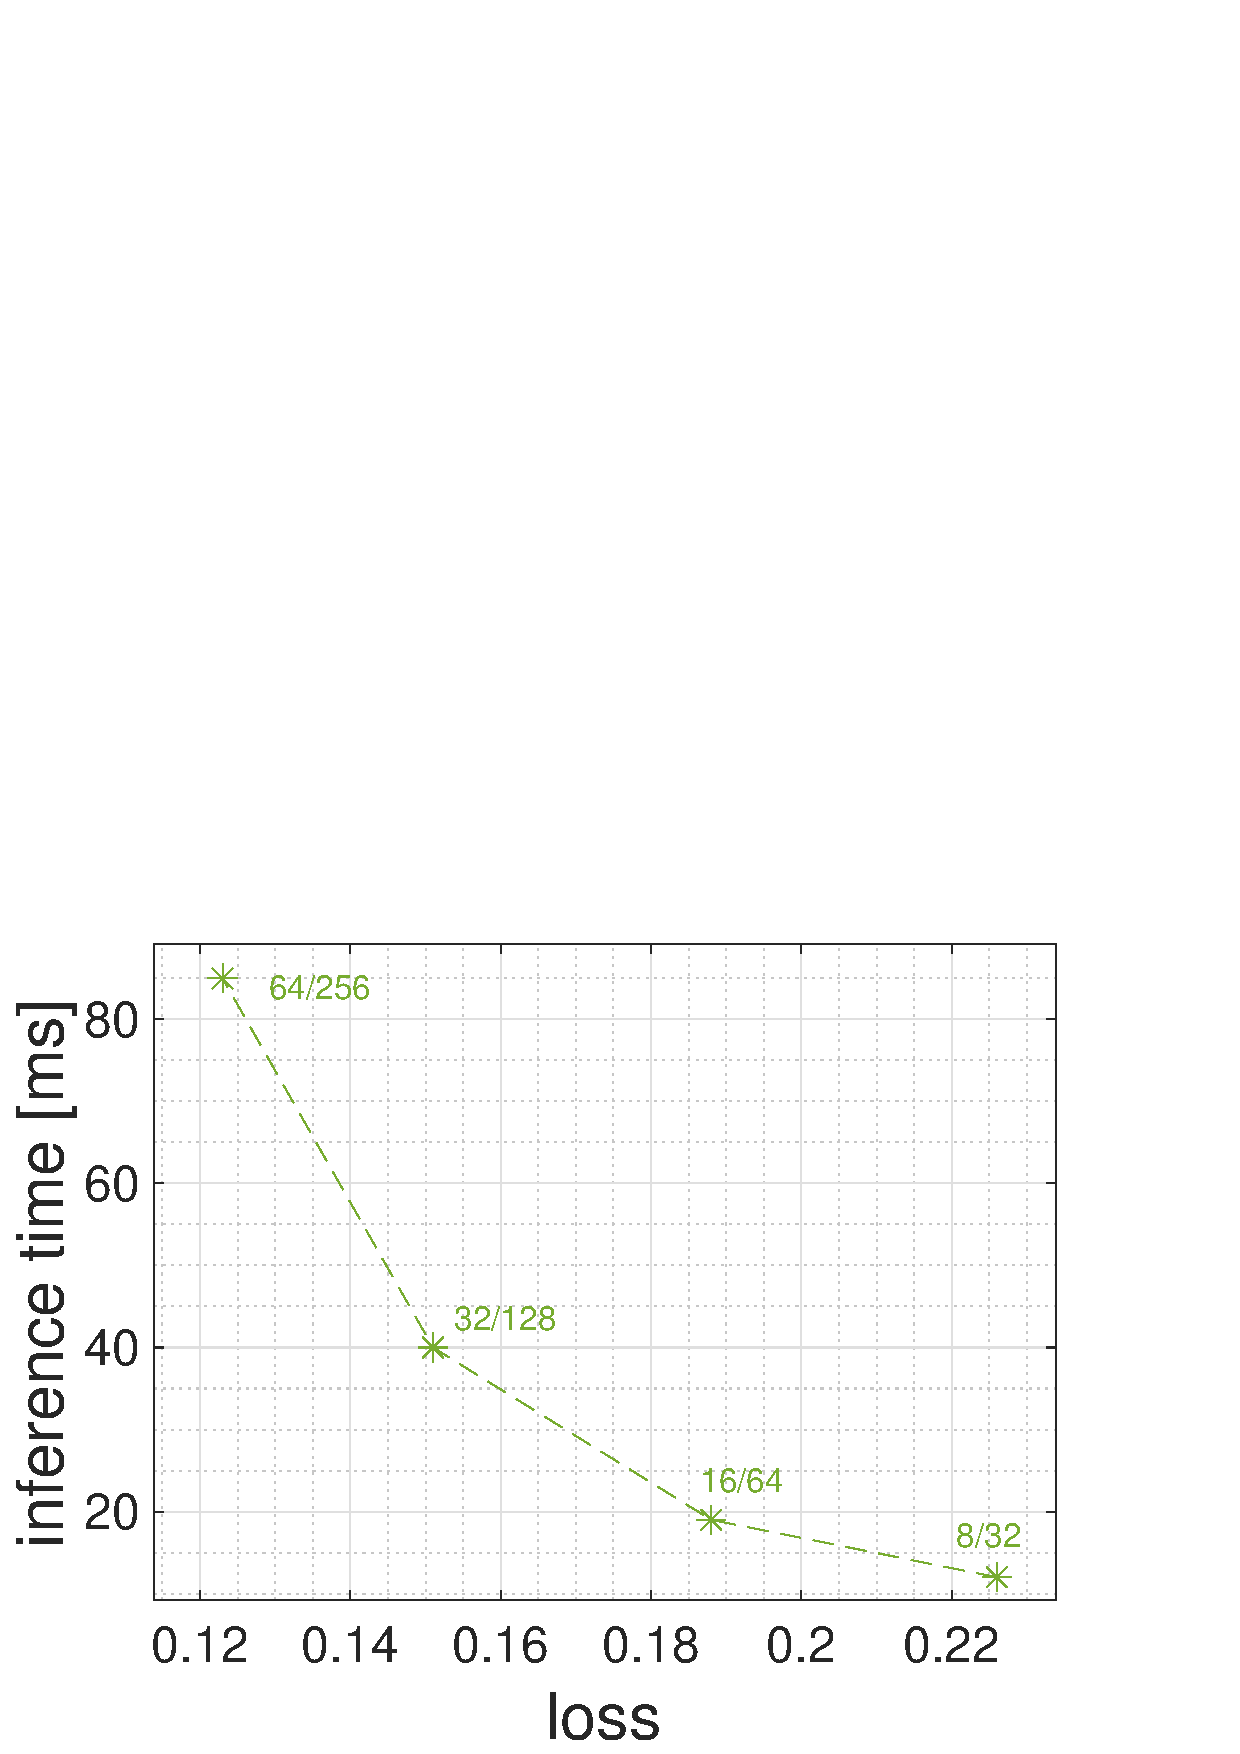
\includegraphics[width=\textwidth]{figure/lstm_time_loss.pdf}
        \caption{tempo d'inferenza vs. loss}
        \label{fig:performance-lstm-hexi:lstm-time-loss}
    \end{subfigure}
    \begin{subfigure}{.45\textwidth}
        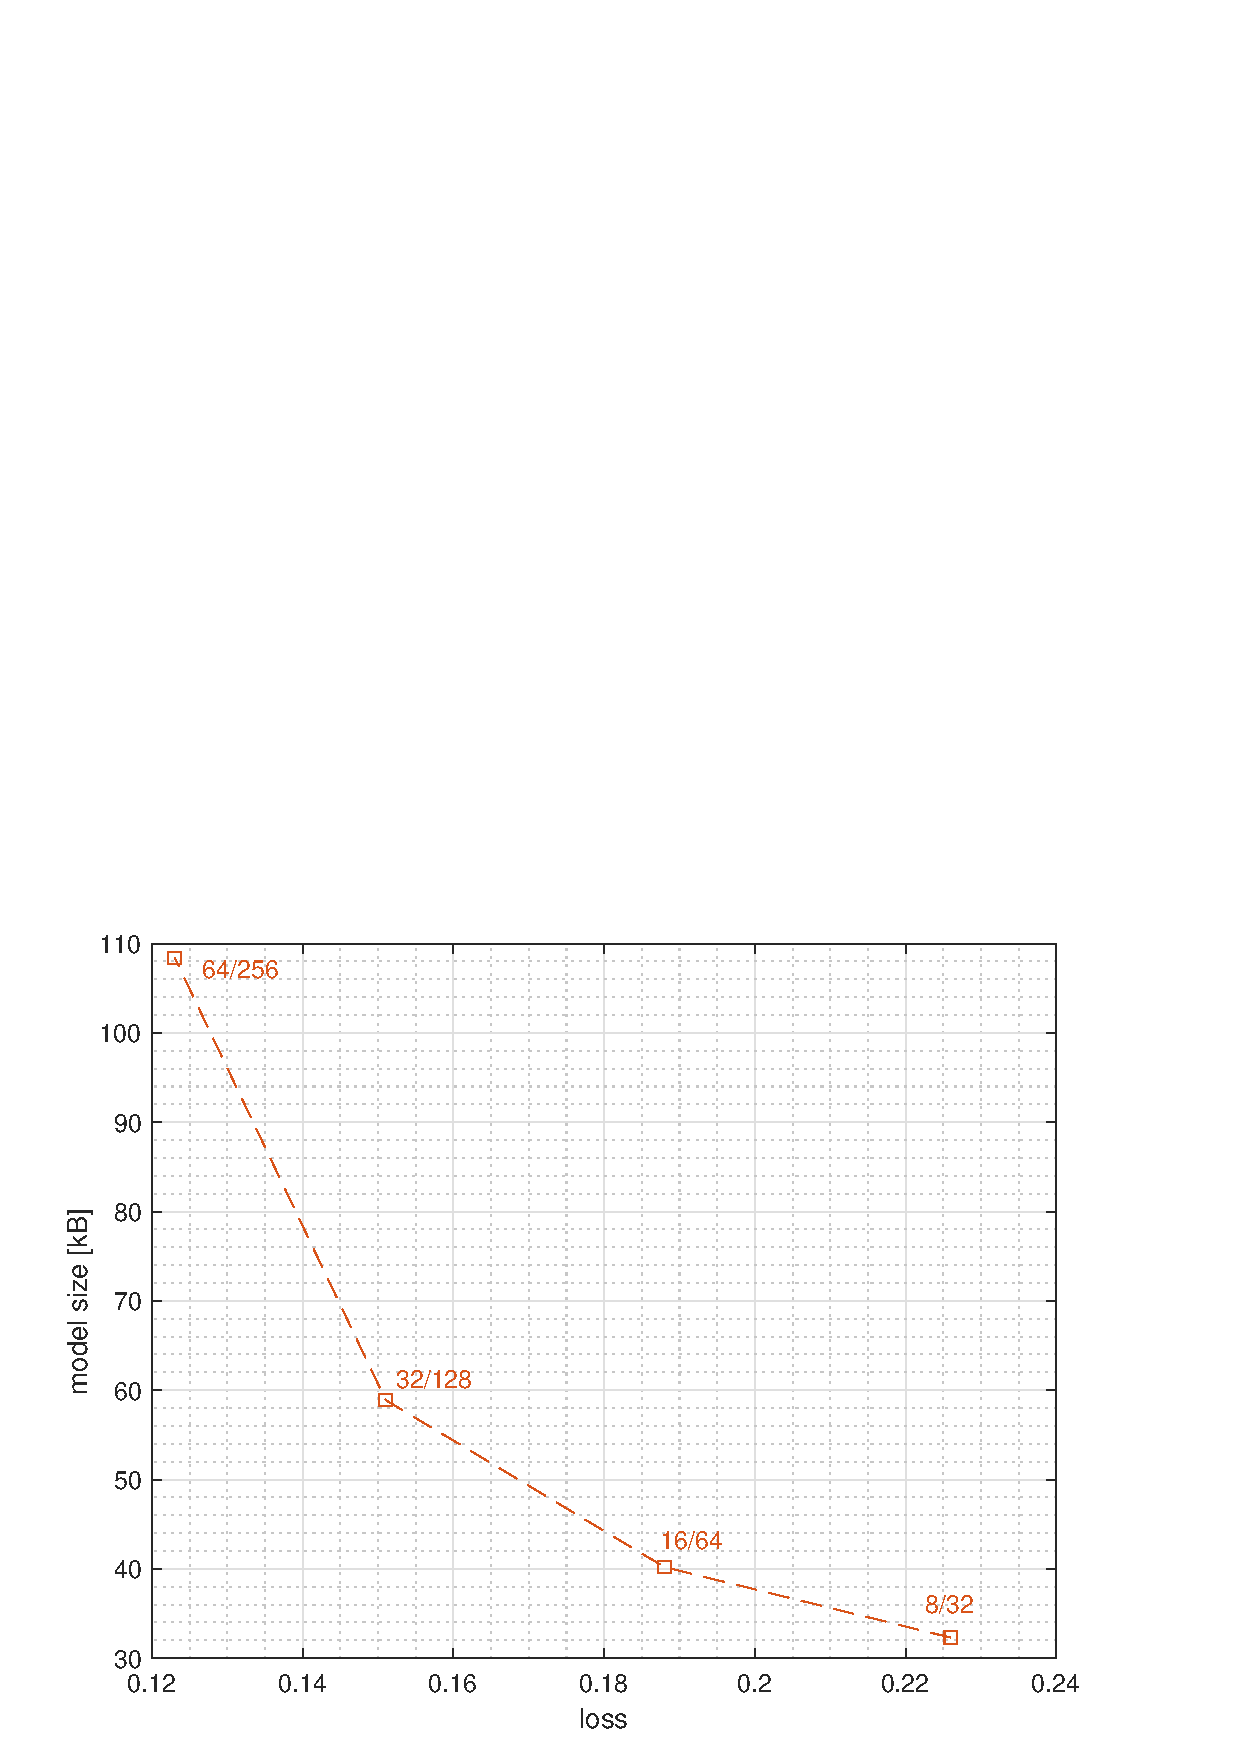
\includegraphics[width=\textwidth]{figure/lstm_size_loss.pdf}
        \caption{dimensione modello vs. loss}
        \label{fig:performance-lstm-hexi:lstm-size-loss}
    \end{subfigure}
    \caption{Grafici prodotti dal modello LSTM confrontando consumo d'energia(\subref{fig:performance-lstm-hexi:lstm-energy-loss}), tempo d'inferenza(\subref{fig:performance-lstm-hexi:lstm-time-loss}) e dimensione modello(\subref{fig:performance-lstm-hexi:lstm-size-loss}) con la loss.}
    \label{fig:performance-lstm-hexi}
\end{figure}

\section{Sviluppo dell'applicazione}
\label{sec:sviluppo-dell-applicazione}

In questa sezione presentiamo lo sviluppo di un'applicazione nativa per lo smartwatch HEXIWEAR. Dopo aver eseguito tutti gli esperimenti sui modelli di machine learning e di deep learning implementati sia su PC che sullo smartwatch abbiamo deciso di sviluppare un'applicazione per l'HEXIWEAR che metta in pratica quanto scoperto in questa tesi ad un contesto comune e più utile per tutti gli utenti. 

L'applicazione sviluppata ha lo scopo di conteggiare il numero di attività di lavaggio e di sanificazione della mani compiute da un utente nell'arco di una giornata; per fare questo raccoglie in maniera continua i valori non elaborati dai sensori di accelerometro e giroscopio ed utilizza uno dei modelli di machine learning visti precedentemente per classificare l'attività svolta. 

L'applicazione nativa è stata sviluppata interamente in C/C++ facendo uso delle API messe a disposizione dal sistema operativo real-time MbedOS; in particolare il processo di build è stato gestito della nuova toolchain CLI \textit{mbed-tools}\cite{mbedtools}, il quale automatizza la fase di building e di flash dell'applicazione e controlla tutti gli aspetti del progetto come rilevare automaticamente i dispositivi embedded connessi o mantenere aggiornate tutte le librerie esterne.

Nell'applicazione sono state utilizzate quattro librerie esterne: le librerie \textit{hexiwear\_FXAS21002}\cite{fxas21002} e \textit{hexiwear\_FXOS8700}\cite{fxos87700} hanno lo scopo di controllare gli omonimi sensori integrati di accelerometro e giroscopio leggendo i loro valori ad una frequenza di 100Hz. La libreria \textit{hexiwear\_KW40Z}\cite{kw40z} consente l'accesso alle funzionalità di Bluetooth Low Energy del micro-processore KW40Z, anche se non è questo il motivo per qui l'abbiamo scelta; infatti questo processore è responsabile anche della gestione di tutti gli eventi provenienti dai bottoni capacitivi posti sulla parte frontale del dispositivo. Infine l'ultima libreria utilizzata è \textit{oled\_ssd1351}\cite{ssd1351} che ha lo scopo di pilotare il display OLED presente sullo smartwatch; a differenza delle altre librerie, create e mantenute dal team di sviluppo dell'HEXIWEAR, questa è stata creata quasi da zero da noi partendo dalla versione ufficiale modificandola pesantemente per adeguarla alle nostre esigenze e risolvere alcuni fastidiosi bug.

\begin{figure}[!htb]
    \centering
    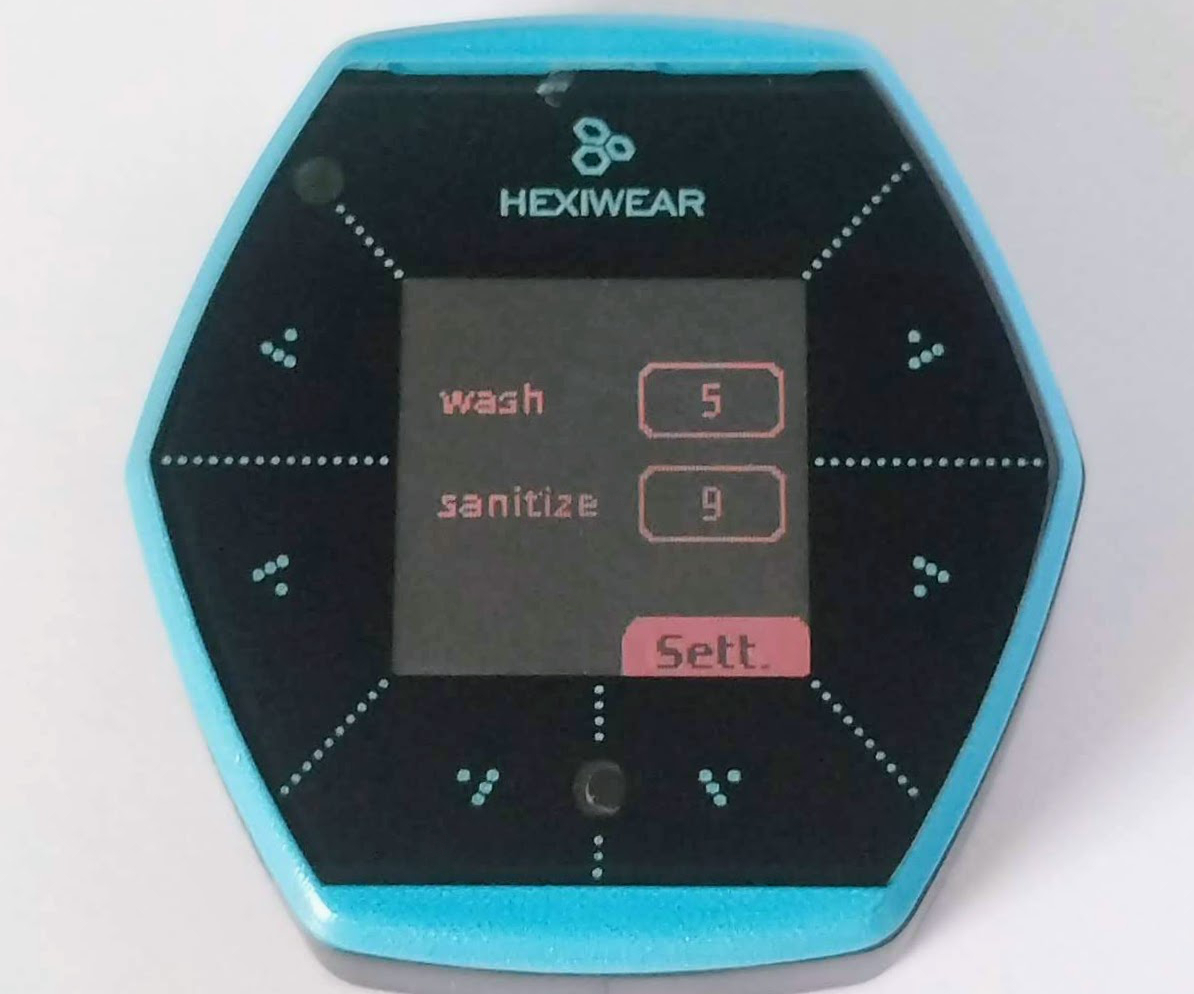
\includegraphics[width=.4\textwidth]{figure/hexiwear-app.jpg}
    \caption{Schermata principale dell'applicazione di monitoraggio delle attività sviluppata per l'HEXIWEAR.}
    \label{fig:hexiwear-app}
\end{figure}

In Figura \ref{fig:hexiwear-app} possiamo vedere la schermata principale dell'applicazione in esecuzione direttamente sul dispositivo HEXIWEAR; il design è semplice, composto da due soli contatori: uno per i lavaggi delle mani ed uno per le sanificazioni. Premendo il pulsante \textit{Settings} saremo portati nella pagina delle impostazioni, nella quale possiamo resettare i contatori a fine giornata.

Per il rilevamento delle attività l'applicazione fa uso del modello di deep learning LSTM presentato nella Sezione \ref{ssec:selezione-dei-parametri-di-lstm-hexi} con i parametri interni settati a 64 unità per il modulo LSTM e 256 neuroni per il primo livello densamente connesso. Si è scelto di utilizzare questa tipologia di rete poiché risulta essere la più prestante in termini delle metriche di accuratezza (tutte le metriche superano l'87\%); inoltre, anche se il tempo d'inferenza e la memoria utilizzata sono maggiori rispetto ai modelli SVM, il consumo d'energia è molto inferiore che, in definitiva, questo parametro non è da trascurare quando si parla di applicazioni embedded o indossabili che hanno bisogno di una lunga durata della batteria.